\documentclass[12pt,a4paper,openany]{book}
\usepackage[utf8]{inputenc}
\usepackage[spanish]{babel}
\usepackage{graphicx}
\usepackage[left=3.0cm,right=3.0cm,top=3.0cm,bottom=3.0cm]{geometry}
\usepackage{mathptmx}
\usepackage{blindtext} 

\usepackage[Glenn]{fncychap} %Estilo para los capitulos, otros pueden ser: Sonny, Lenny, Glenn, Conny, Rejne, Bjarne, Bjornstrup

\usepackage{amssymb, amsmath, amsbsy, amsfonts}    % ECUACIONES Y SÍMBOLOS MATEMÁTICOS
\usepackage{listings} % PERMITE AGREGAR CÓDIGO DE LENGUAJES  DE PROGRAMACIÓN (DOCUMENTACIÓN EN GOOGLE)
\usepackage{emptypage}                   % QUITA LOS ENCABEZADOS Y PIES DE PÁGINA EN LAS HOJAS VACÍAS PRODUCIDAS POR LA IMPRESIÓN A DOS CARAS
\usepackage{wrapfig}                    % to include figure with text wrapping around it
\usepackage[bf,SL,BF]{subfigure}         % Permite crear figuras múltiples
\usepackage{makeidx}                     % Contiene los macros para indexar en un glosario
\usepackage{mathdots}                    % para el comando \iddots
\usepackage{mathrsfs}                    % para formato de letra en ecuaciones
\raggedbottom                            %Evita que LaTeX distribuya los espacios en blanco sobre la página, en lugar de eso los envía al fondo
\usepackage{eucal}
\usepackage{float}
\usepackage{color}
\usepackage[perpage]{footmisc}
\usepackage{ifthen}
\usepackage{multicol} % for pages with multiple text columns, e.g. References
\setlength{\columnsep}{20pt} % space between columns; default 10pt quite narrow
\usepackage[nottoc]{tocbibind} % correct page numbers for bib in TOC, nottoc suppresses an entry for TOC itself
%\usepackage{nextpage}
% \usepackage{titlesec}
%\usepackage[siunitx]{circuitikz} %para circuitos
%\usepackage[makeroom]{cancel}%Para cancelar términos en modo matemático
%\usepackage{cleveref}           %COMO UNA FORMA DE REFERENCIAR TABLAS, ECUACIONES, ETC. -->http://mirror.utexas.edu/ctan/macros/latex/contrib/cleveref/cleveref.pdf
\pagenumbering{roman}

%%%%%%%%%%%%%%%%%%%%%%%%%%%%%%%%%%%%%%%%%%%%%%%%%%%%%%%%%%%%%%%%%%%%%%%%%%%%%%%%
%                                   DATOS                                      %
%%%%%%%%%%%%%%%%%%%%%%%%%%%%%%%%%%%%%%%%%%%%%%%%%%%%%%%%%%%%%%%%%%%%%%%%%%%%%%%%
\author{Marco Antonio Aguilar Gallardo}
\title{Tesis UNAQ}



\begin{document}
\frontmatter
%%%%%%%%%%%%%%%%%%%%%%%%%%%%%%%%%%%%%%%%%%%%%%%%%%%%%
%                   PORTADA                         %
%%%%%%%%%%%%%%%%%%%%%%%%%%%%%%%%%%%%%%%%%%%%%%%%%%%%%

\begin{titlepage}
	\begin{center}
		{\Huge Universidad Aeronáutica en Querétaro}
		\vspace{1cm}
		\begin{figure}[h]
			\centering
			
\includegraphics[scale=0.5]{Portada/Logo.eps}
		\end{figure}
		\vspace{1cm}
		{\large Innovación educativa para el desarrollo de México}
		\vspace{0.5cm}
		\rule{150mm}{0.5mm}
		\vspace{2mm}
		{\huge TESIS}
		\vspace{2mm}
		\rule{150mm}{0.5mm}
		\vspace{1cm}
		\large Trabajo Profesional para obtener el Titulo de Ingeniero en Electrónica y Control de Sistemas de Aeronaves.
		\\
		\vspace{1cm}
		\Large Marco Antonio Aguilar Gallardo
		\\
		\vspace{1cm}
		\Large Dirige: Antonio Flores 
		\vfill
		\Large Municipio de Colón, Querétaro \hfill \today
		
		
	\end{center}


\clearpage

\end{titlepage}


%%%%%%%%%%%%%%%%%%%%%%%%%%%%%%%%%%%%%%%%%%%%%%%%%%%%%
%                  PRÓLOGO                          %
%%%%%%%%%%%%%%%%%%%%%%%%%%%%%%%%%%%%%%%%%%%%%%%%%%%%%
\begin{dedication}
A la Facultad de Ingeniería y a la  Universidad, por la formación que me han dado.\\
Es gracias a ustedes que es posible el presente trabajo.\\
En verdad, gracias.\\
Yo.
\end{dedication}

\chapter{Agradecimientos}

%%%%%%%%%%%%%%%%%%%%%%%%%%%%%%%%%%%%%%%%%%%%%%%%%%%%%
%                   ÍNDICES                         %
%%%%%%%%%%%%%%%%%%%%%%%%%%%%%%%%%%%%%%%%%%%%%%%%%%%%%
%Esta sección genera el índice
\setcounter{secnumdepth}{3} % organisational level that receives a numbers
\setcounter{tocdepth}{3}    % print table of contents for level 3
% \tableofcontents            % Genera el índice 
%: ----------------------- list of figures/tables ------------------------
\listoffigures              % Genera el ínidce de figuras, comentar línea si no se usa
\listoftables               % Genera índice de tablas, comentar línea si no se usa

%%%%%%%%%%%%%%%%%%%%%%%%%%%%%%%%%%%%%%%%%%%%%%%%%%%%%
%                   CONTENIDO                       %
%%%%%%%%%%%%%%%%%%%%%%%%%%%%%%%%%%%%%%%%%%%%%%%%%%%%%
\mainmatter
\chapter{Introducción}
En el presente capitulo se expone el objetivo general, así como sus derivados. En la
primera sección se aborda el tema de investigación donde especifica la justificación del
presente trabajo, posteriormente se sintetiza algunas de las investigaciones que sirvieron
como base para la elección del tema previamente descrito. Finalmente se dan las razones
de la investigación y se exponen las aportaciones derivadas del tema de tesis.

\section{Tema de investigación}
En el campo de la aeronáutica hay una rama que en los últimos años ha sido objeto
de estudio debido a su exponencial importancia para tareas criticas, se trata de los
vehículos aéreos no tripulados UAV (del inglés unmanned aerial vehicle), donde dichas 
tareas criticas han podido alcanzar sus objetivos en parte gracias a la implementación
reciente de visión artificial, que dicho sea de paso ha dado pie a múltiples investigaciones
para generar una buena comunicación de datos entre el UAV y un sistema receptor en
tierra, dado que aveces las tareas requieren un tiempo de respuesta menor del que un
protocolo de comunicación puede otorgar o en donde se necesita garantizar la seguridad
tanto de software y hardware ha surgido la necesidad de diseñar un sistema embebido
con la finalidad de evitar los problemas relacionados con los protocolos de comunicación
y a su vez tener como resultado un sistema enteramente autónomo.

\section{Justificación}


\section{Objetivo}
%%%%%%%%%%%%%%%%%%%%%%%%%%%%%%%%%%%%%%%%%%%%%%%%%%%%%%%%%%%%%%%%%%%%%%%%%
%Se escribe en infinitivo y resuelve las preguntas ¿Que? ¡Como? y ¿para que? %
%%%%%%%%%%%%%%%%%%%%%%%%%%%%%%%%%%%%%%%%%%%%%%%%%%%%%%%%%%%%%%%%%%%%%%%%%
Diseñar, instrumentar y controlar un dispositivo gimbal que sea capaz de seguir un objeto a través de visión artificial para implementarse en un UAV de categoría pequeña a velocidad baja.

\section{Objetivos específicos}
%%%%%%%%%%%%%%%%%%%%%%%%%%%%%%%%%%%%%%%%%%%%%%%%%%%%%%%%%%%%%%%%%%%%%%%%%
%Seran los capitulos de la tesis %
%%%%%%%%%%%%%%%%%%%%%%%%%%%%%%%%%%%%%%%%%%%%%%%%%%%%%%%%%%%%%%%%%%%%%%%%%
\begin{itemize}
    \item Obtener el modelo matemático de una gimbal de 2 grados de libertad.
    \item Diseñar e implementar el sistema embebido que dará el soporte electrónico a la gimbal.
    \item Capturar figuras geométricas definidas  mediante el uso de una cámara digital y emplear algoritmos de visión artificial para la obtención de datos. 
    \item Diseñar un controlador autónomo con base en el modelo matemático, previamente obtenido.
    \end{itemize}

\section{Estado de la cuestion}
%%%%%%%%%%%%%%%%%%%%%%%%%%%%%%%%%%%%%%%%%%%%%%%%%%%%%%%%%%%%%%%%%%%%%%%%%
%Descripción breve de las obras, proyectos, intentos universitarios más significativos %
%%%%%%%%%%%%%%%%%%%%%%%%%%%%%%%%%%%%%%%%%%%%%%%%%%%%%%%%%%%%%%%%%%%%%%%%%
La aparición de la gimbal no es un termino para nada nuevo, de hecho es viejo más de lo que
muchos podemos creer. Fue en el 250 antes de nuestra era cuando el inventor Philo of Byzantium
describió un bote de tinta de ocho lados con una abertura en cada lado, que se puede
girar de modo que mientras cualquier cara está en la parte superior, se puede sumergir y
entintar un bolígrafo, aunque la tinta nunca se agota a través de los agujeros de los otros
lados.~\cite{Gimbal}.\\
Desde entonces y hasta la fecha múltiples científicos han desarrollado investigaciones alrededor
de dicho artefacto, algunos teniendo más éxito que otros; los cuales serán brevemente expuestos
con la finalidad de obtener el estado actual en el que se encuentra la gimbal y su avance
tecnológico.
\begin{itemize}
    \item \textbf{Navegación inercial}\\
    En la navegación inercial, como se aplica a los barcos y submarinos, se necesita 
    un mínimo de tres gimbals para permitir que un sistema de navegación inercial 
    (masa estable) permanezca fijo en el espacio inercial, compensando los cambios 
    en el guiñada, inclinación y balanceo del barco.
    \begin{center}
        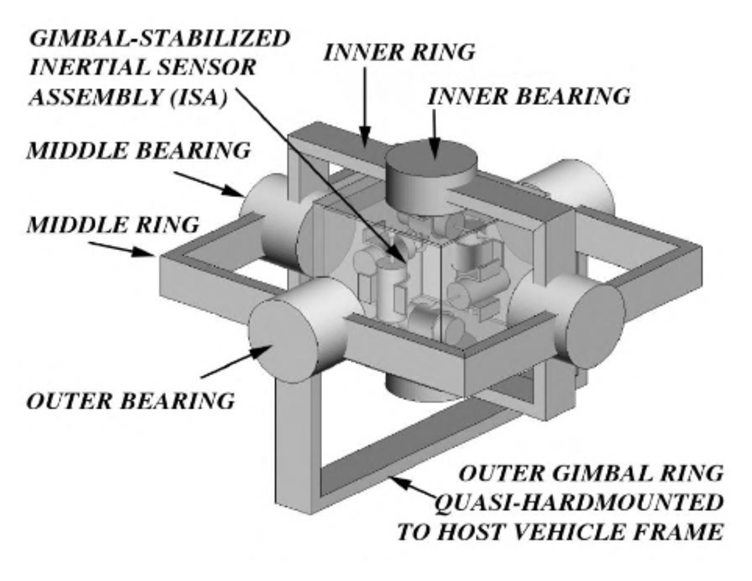
\includegraphics[width=0.6\textwidth]{Capitulo1/Fig1.eps}       
        \captionof{figure}{Uso de una gimbal para una IMU ~\cite{InertialNavigation} }\label{Fig1}
    \end{center}
    En esta aplicación, la Unidad de medición inercial (IMU) está equipada con tres 
    giroscopios montados ortogonalmente para detectar la rotación alrededor de todos 
    los ejes en el espacio tridimensional. Las salidas giroscópicas accionan motores 
    que controlan la orientación de los tres gimbal según sea necesario para mantener 
    la orientación de la IMU.

    \item \textbf{Motores de cohete}\\
    En la propulsión de naves espaciales, los motores de cohetes generalmente se 
    montan en un par de gimbals para permitir que un solo motor logre el empuje 
    sobre los ejes de inclinación y guiñada; o, a veces, solo se proporciona un eje 
    por motor. Para controlar el giro, se utilizan motores gemelos con señales de 
    control de inclinación diferencial o guiñada para proporcionar torque sobre el 
    eje de balanceo del vehículo.\\
    Uno de los motores más famosos es el J-2X.Es un motor de cohete avanzado altamente 
    eficiente y versátil con las características ideales de empuje y rendimiento para 
    impulsar la etapa superior del espacio de la NASA.~\cite{NASA}
    \begin{center}
        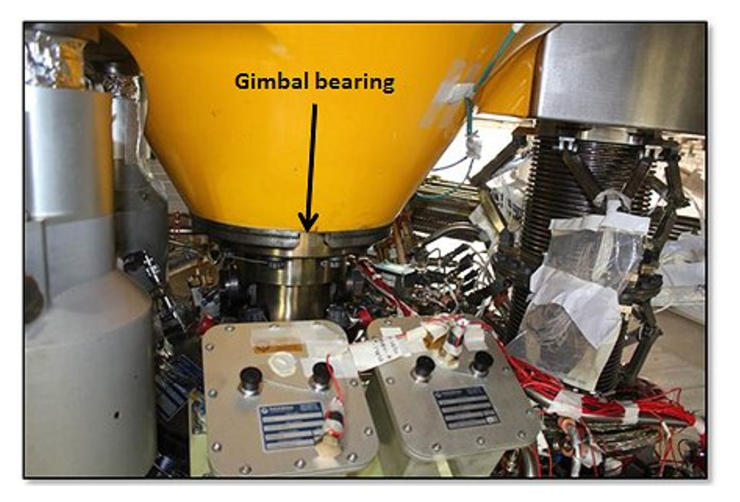
\includegraphics[width=0.6\textwidth]{Capitulo1/Fig2.eps}       
        \captionof{figure}{Uso de una gimbal en un motor de propulsión ~\cite{NASA2JX} }\label{Fig2}
    \end{center}

    \item \textbf{Entrenamiento para astronautas}\\
    Sistema de simulación de maniobras de tipo caída que se pueden encontrar en el vuelo espacial
    fue creado por la NASA y era conocido como "the gimbal rig,".
    Tres jaulas tubulares de aluminio podrían girar por separado o en combinación para 
    dar movimientos de balanceo, cabeceo y guiñada a velocidades de hasta 30 
    revoluciones por minuto, mayores que las esperadas en vuelos espaciales reales. 
    Los chorros de gas nitrógeno, unidos a las tres jaulas, controlaron el movimiento.
    Desde el 15 de febrero hasta el 4 de marzo de 1960, la plataforma de cardán 
    proporcionó una capacitación valiosa para los siete astronautas del Proyecto 
    Mercurio. Cada uno experimentó unas cinco horas de tiempo de vuelo simulado.
    ~\cite{MERCURY}
    \begin{center}
        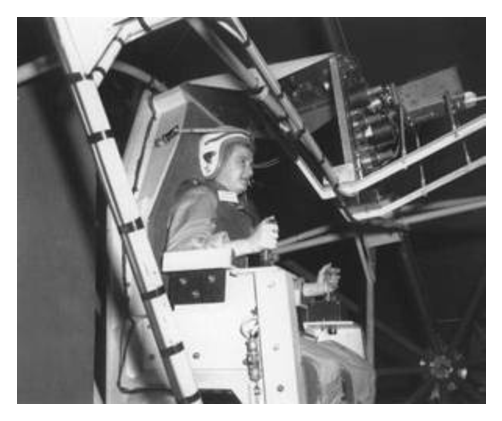
\includegraphics[width=0.6\textwidth]{Capitulo1/Fig3.eps}       
        \captionof{figure}{Jerrie Cobb, uno de los Mercury 13, da un giro en la plataforma gimbal.
        Créditos: NASA }\label{Fig3}
    \end{center}

    \item \textbf{Estabilizador de Camaras}\\
    Los gimbals también se utilizan para montar todo, desde lentes de cámara pequeñas 
    hasta telescopios fotográficos grandes.\\
    En los equipos de fotografía portátiles, se utilizan gimbals de un 
    solo eje para permitir un movimiento equilibrado de la cámara y las lentes. 
    Esto resulta útil en la fotografía semi-profesional, así como en cualquier otro 
    caso en el que se adopten teleobjetivos muy largos y pesados: un eje de la gimbal 
    gira un lente alrededor de su centro de gravedad, lo que permite una manipulación 
    fácil y suave mientras se rastrea a los sujetos en movimiento.\\
    Los montajes de gimbal muy grandes en forma de montajes de altitud-altitud de 2 o 3 ejes 
    se utilizan en la fotografía satelital con fines de seguimiento.\\
    En la década de 1970, el director de fotografía estadounidense Garrett Brown tuvo 
    una idea simple pero revolucionaria: hacer un dispositivo que pudiera suavizar las 
    tomas de acción manuales. 
    \begin{center}
        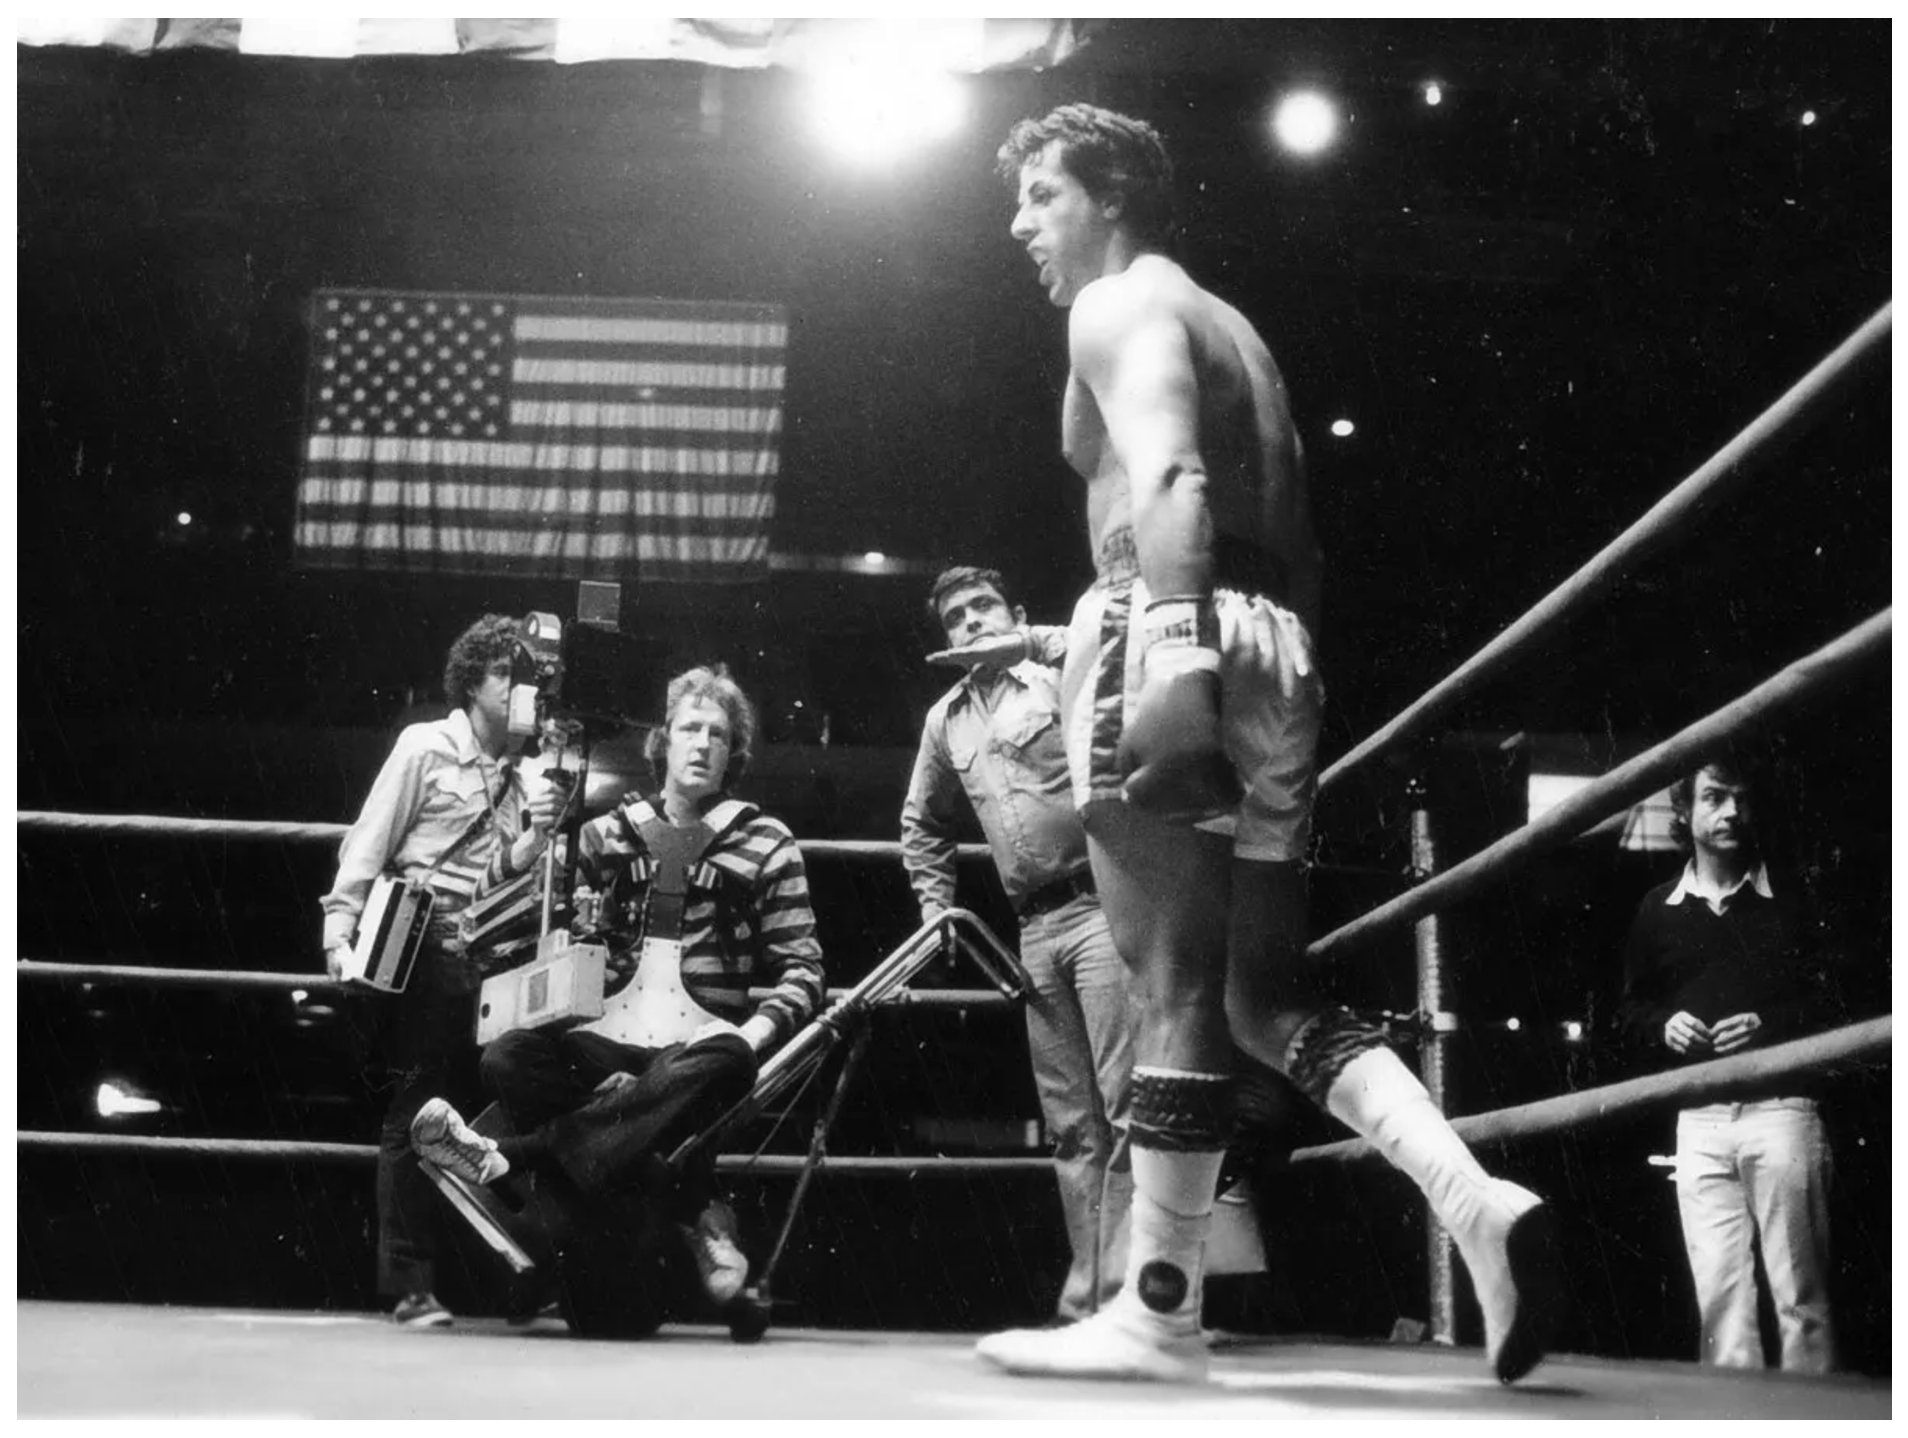
\includegraphics[width=0.5\textwidth]{Capitulo1/Fig4.eps}       
        \captionof{figure}{Primer uso de la steadicam}\label{Fig4}
    \end{center}

    El resultado es el Steadicam (Que cumple con los principios físicos de la gimbal) \\
    Ganador de un Premio de la Academia, que hizo su debut cinematográfico en la 
    película "Bound for Glory", y se destacó en las películas "Rocky" y "The Shining"


\end{itemize}

\section{Contribuciones}
%%%%%%%%%%%%%%%%%%%%%%%%%%%%%%%%%%%%%%%%%%%%%%%%%%%%%%%%%%%%%%%%%%%%%%%%%
%                         Contribuciones                                %
%%%%%%%%%%%%%%%%%%%%%%%%%%%%%%%%%%%%%%%%%%%%%%%%%%%%%%%%%%%%%%%%%%%%%%%%%

\section{Alcances}
%%%%%%%%%%%%%%%%%%%%%%%%%%%%%%%%%%%%%%%%%%%%%%%%%%%%%%%%%%%%%%%%%%%%%%%%%
%¿Porque es relevante la solucion o mejora o implementacion.? ¿por que es novedosa? %
%%%%%%%%%%%%%%%%%%%%%%%%%%%%%%%%%%%%%%%%%%%%%%%%%%%%%%%%%%%%%%%%%%%%%%%%%


\section{Estructura de la tesis}



%%%%%%%%%%%%%%%%%%%%%%%%%%%%%%%%%%%%%%%%%%%%%%%%%%%%%
%                   REFERENCIAS                     %
%%%%%%%%%%%%%%%%%%%%%%%%%%%%%%%%%%%%%%%%%%%%%%%%%%%%%
\backmatter

% existen varios estilos de bilbiografía, pueden cambiarlos a placer
\bibliographystyle{apalike} % otros estilos pueden ser abbrv, acm, alpha, apalike, ieeetr, plain, siam, unsrt

\end{document}